\documentclass[a0paper,portrait]{baposter}
\usepackage{CJKutf8} %% 中文套件

\usepackage{relsize}		% For \smaller
\usepackage{url}			% For \url
\usepackage{epstopdf}	% Included EPS files automatically converted to PDF to include with pdflatex

%%% Global Settings %%%%%%%%%%%%%%%%%%%%%%%%%%%%%%%%%%%%%%%%%%%%%%%%%%%%%%%%%%%

\graphicspath{{pix/}}	% Root directory of the pictures 
% \tracingstats=2			% Enabled LaTeX logging with conditionals

%%% Color Definitions %%%%%%%%%%%%%%%%%%%%%%%%%%%%%%%%%%%%%%%%%%%%%%%%%%%%%%%%%

\definecolor{bordercol}{RGB}{40,40,40}
\definecolor{headercol1}{RGB}{186,215,230}
\definecolor{headercol2}{RGB}{80,80,80}
\definecolor{headerfontcol}{RGB}{0,0,0}
\definecolor{boxcolor}{RGB}{186,215,230}

%%%%%%%%%%%%%%%%%%%%%%%%%%%%%%%%%%%%%%%%%%%%%%%%%%%%%%%%%%%%%%%%%%%%%%%%%%%%%%%%
%%% Utility functions %%%%%%%%%%%%%%%%%%%%%%%%%%%%%%%%%%%%%%%%%%%%%%%%%%%%%%%%%%

%%% Save space in lists. Use this after the opening of the list %%%%%%%%%%%%%%%%
\newcommand{\compresslist}{
	\setlength{\itemsep}{1pt}
	\setlength{\parskip}{0pt}
	\setlength{\parsep}{0pt}
}

%%%%%%%%%%%%%%%%%%%%%%%%%%%%%%%%%%%%%%%%%%%%%%%%%%%%%%%%%%%%%%%%%%%%%%%%%%%%%%%
%%% Document Start %%%%%%%%%%%%%%%%%%%%%%%%%%%%%%%%%%%%%%%%%%%%%%%%%%%%%%%%%%%%
%%%%%%%%%%%%%%%%%%%%%%%%%%%%%%%%%%%%%%%%%%%%%%%%%%%%%%%%%%%%%%%%%%%%%%%%%%%%%%%

\begin{document}
\begin{CJK*}{UTF8}{bsmi}
\typeout{Poster rendering started}

%%% Setting Background Image %%%%%%%%%%%%%%%%%%%%%%%%%%%%%%%%%%%%%%%%%%%%%%%%%%
\background{
	\begin{tikzpicture}[remember picture,overlay]%
	\draw (current page.north west)+(-2em,2em) node[anchor=north west]
	{
\includegraphics[height=1.1\textheight]{background}};
	\end{tikzpicture}
}

%%% General Poster Settings %%%%%%%%%%%%%%%%%%%%%%%%%%%%%%%%%%%%%%%%%%%%%%%%%%%
%%%%%% Eye Catcher, Title, Authors and University Images %%%%%%%%%%%%%%%%%%%%%%
\begin{poster}{
	grid=false,
	% Option is left on true though the eyecatcher is not used. The reason is
	% that we have a bit nicer looking title and author formatting in the headercol
	% this way
	%eyecatcher=false, 
	borderColor=bordercol,
	headerColorOne=headercol1,
	headerColorTwo=headercol2,
	headerFontColor=headerfontcol,
	% Only simple background color used, no shading, so boxColorTwo isn't necessary
	boxColorOne=boxcolor,
	headershape=roundedright,
	headerfont=\Large\sf\bf,
	textborder=rectangle,
	background=user,
	headerborder=open,
  boxshade=plain
}
%%% Eye Cacther %%%%%%%%%%%%%%%%%%%%%%%%%%%%%%%%%%%%%%%%%%%%%%%%%%%%%%%%%%%%%%%
{
	Eye Catcher, empty if option eyecatcher=false - unused
}
%%% Title %%%%%%%%%%%%%%%%%%%%%%%%%%%%%%%%%%%%%%%%%%%%%%%%%%%%%%%%%%%%%%%%%%%%%
{\sf\bf
    Application of CNN and WSNs for Epidemic Prevention
}
%%% Authors %%%%%%%%%%%%%%%%%%%%%%%%%%%%%%%%%%%%%%%%%%%%%%%%%%%%%%%%%%%%%%%%%%%
{
    \vspace{1em} \textbf{Advisor: Prof. Gwo-Jong Yu} \\
	\textbf{Students: Wei-Chun Tsai, Yang Yang, Shin-Hua Lee} \\
	
}
%%% Logo %%%%%%%%%%%%%%%%%%%%%%%%%%%%%%%%%%%%%%%%%%%%%%%%%%%%%%%%%%%%%%%%%%%%%%


\headerbox{Abstract(摘要)}{name=Abstract,column=0,row=0}{
COVID-19 (新型冠狀病毒) disease has since spread worldwide, leading to an ongoing pandemic since 2020. In this project, constructed a system that is at a low cost by using \textbf{Android APP}, \textbf{MLX90614} and \textbf{RFID} with a \textbf{Buzzer}. Which can be set up on the public transportation. 
}

\headerbox{Statement of Problems}{name=SOP,column=0,below=Abstract}{
COVID-19 was an infectious disease caused by the SARS-CoV-2 virus since 2019. Because none of the strategies for epidemic prevention was cheap (大眾交通工具上沒有一項便宜的防疫產品), therefore, the system was built. To prevent epidemic at a low cost in public transportation.
}

\headerbox{Neural Networks Training}{name=models,column=0,below=SOP}{
After using \textbf{Convolution Neural Networks} and \textbf{Caffe Model} training with \textbf{20 epochs}, received the highest validation accuracy (驗證準確度) of face-mask wearing detection.
\begin{center}
    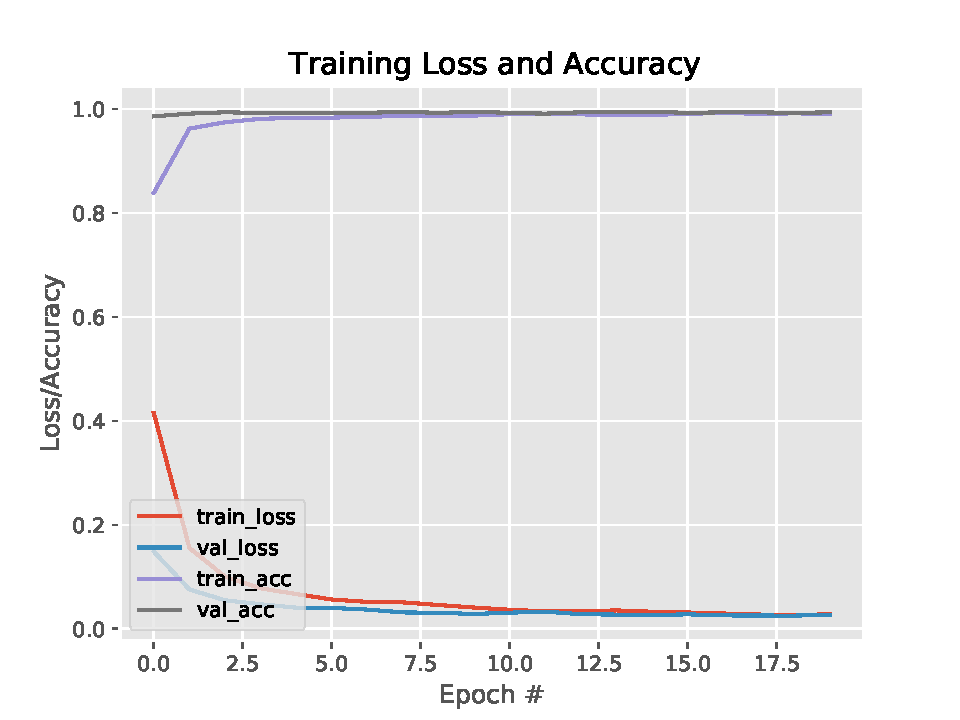
\includegraphics[scale=0.42]{plot.pdf}
\end{center}
}

\headerbox{Conclusion(結論)}{name=Conclusion,column=0,below=models}{
COVID-19 must have had a considerable impact on the world since 2020. The core values of this system are \textit{low cost} (低成本) and \textit{machine vision} (電腦視覺). This system can be said to be a weapon in epidemic prevention of public transportation! (大眾交通工具防疫系統)
}

\headerbox{Members(團隊介紹)}{name=members,column=0,below=Conclusion, above=bottom}{

\vspace{0.4em}			% Save some space at the beginning
\hspace{1em}\textbf{Prof. Gwo-Jong Yu} (游國忠\quad博士), he is currently a Professor in Aletheia University. His current research interests include Mobile Networks, Machine Learning, Big Data, Deep Learning, Digital Image Processing. \\

\hspace{1em}\textbf{Wei-Chun Tsai} (蔡煒俊), he is currently a full-time software engineer in Academia Sinica. His research interests include Digital Image Processing, Artificial Intelligence, Deep Learning, Autonomous Cars, Multimedia Big Data Computing. \\

\hspace{1em}\textbf{Yang Yang} (楊暘), his research interests include RFID, Embedded Systems, Internet of Things, Integrated Circuit Design. \\

\hspace{1em}\textbf{Shin-Hua Lee} (李昕樺), his research interests include Embedded Systems, Wireless Sensor Networks, Internet of Things, Integrated Circuit Design.
}

\headerbox{Thematic Results(研究成果)}{name=Result,span=2,column=1,row=0}{ %% needs to update
\begin{center}
    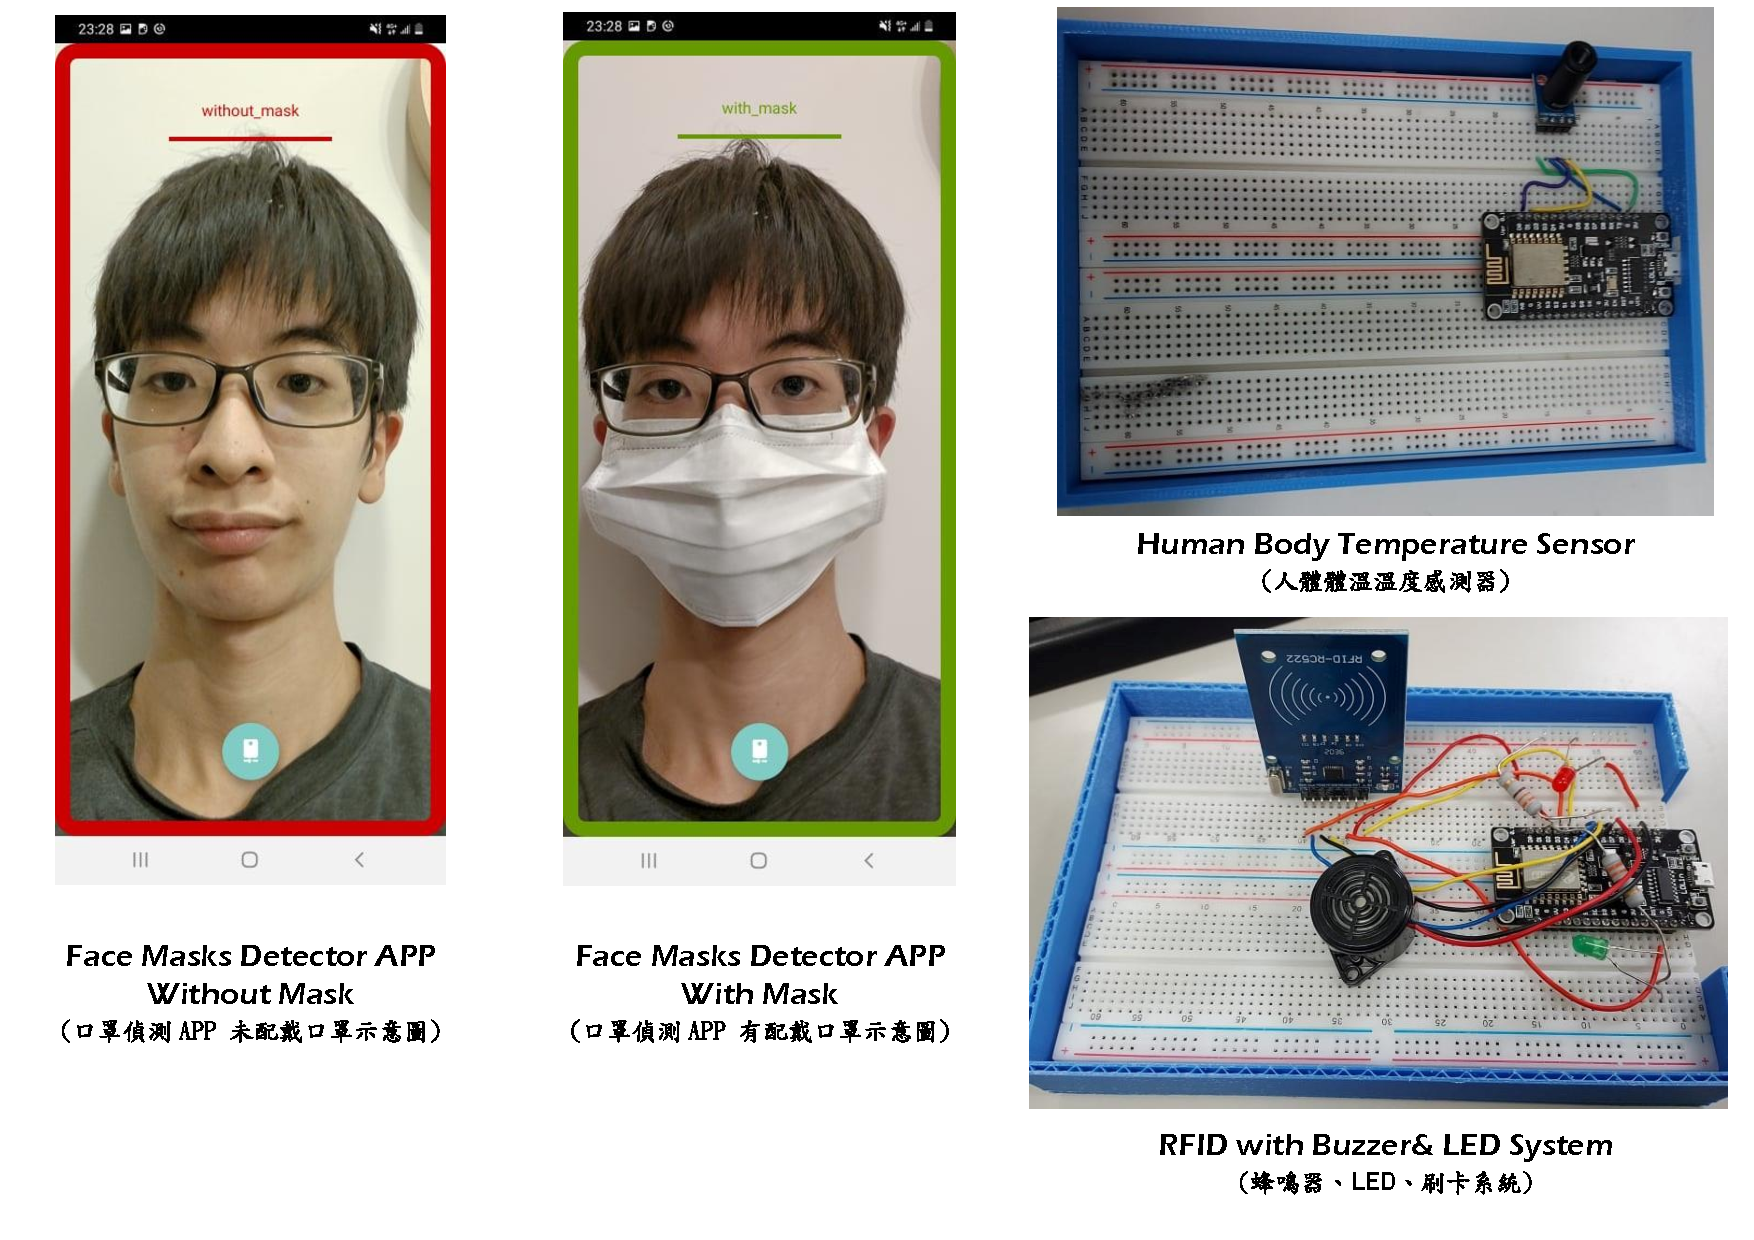
\includegraphics[scale=0.52]{System.pdf}
\end{center}
} %% needs to update

\headerbox{Method and Process(實作方法與步驟)}
{name=MP,span=2,column=1,below=Result,above=bottom}{
\textbf{First, a passenger walks through the doorway and swipes an RFID card(首先刷卡). After swiping the RFID card, \textit{Epidemic Prevention Inspector}(打開防疫督察官) will open the Android APP for face-mask detection(檢查口袋配戴) and open MLX90614 for the human body temperature measuring(體溫量測). If both face-mask detection and human body temperature are ok, the buzzer will buzz not sound but LED will be blinked(都符合標準,LED 會閃爍). That is to say,  either human body temperature not ok or face mask was not wearing, the buzzer will buzz for a specific sound(其一不符合標準,蜂鳴器會叫出特定聲音). In this case, the communication method of our system's integration is using MQTT. (此系統串接與整合是使用MQTT)} \\
\begin{center}
    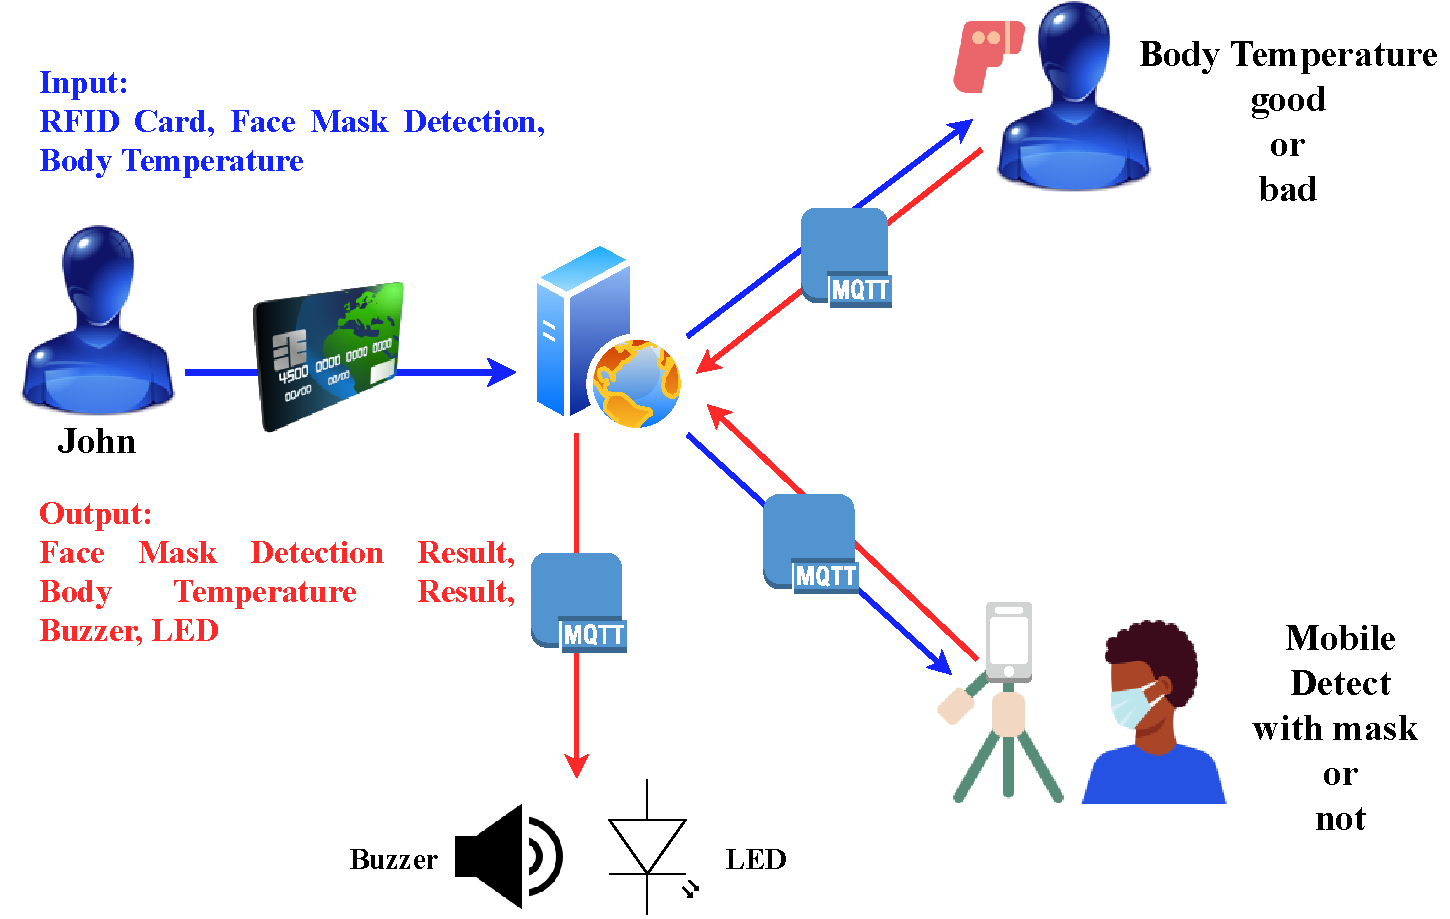
\includegraphics[scale=0.6]{FlowChart.pdf} \\
\end{center}
\begin{center}
    \textbf{\textit{Architecture of Epidemic Prevention Inspector}}
\end{center}
}

\end{poster}
\end{CJK*}
\end{document}
